\section{姿勢制御試験}

本衛星は,搭載した永久磁石により,地磁気の磁力線に沿う様に回転する.本
試験では,EMが正しく磁力線方向に姿勢を変更するかの確認を行った.試験の
実施方法としては.水を張ったプールの上に発泡スチロールの板を浮かべ,そ
の上に防水パックに封入した衛星EMを載せて自由回転させた.運動の様子を図
\ref{4_6_mag_exp1}に示す.尚,ヒステリシスダンパの効果については,水や
空気の抵抗・粘性よりも発生力が小さいため,確認していない.


\begin{figure}[htbp]
	\centering
	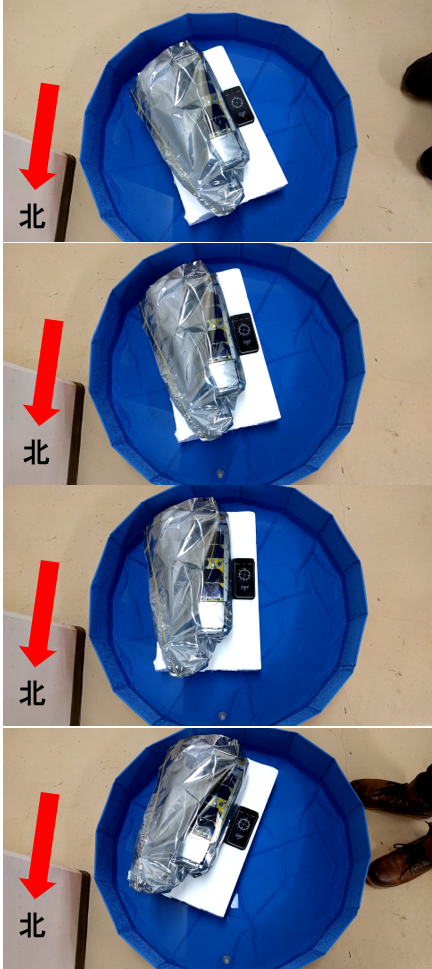
\includegraphics[width=10cm]{./04/fig/4_6_mag1.png}
	\caption{磁力による姿勢変更実験}
	\label{4_6_mag_exp}
\end{figure}
